\documentclass[20pt]{beamer}
\usepackage[utf8]{inputenc}
\usepackage[T1]{fontenc}
\usepackage{lmodern}
\usepackage{graphicx}
\usetheme{default}
\usepackage{tabulary}


\newcommand\e{\emph}
\newcommand\tb{\textbf}
\newcommand\un{\underline}
\newcommand\txt{\texttt}


\begin{document}
	\author{Jennifer Lin}
	\title{Place of Residence and Political Attitudes in Democracies Worldwide}
	%\subtitle{}
	%\logo{}
	%\institute{New College of Florida}
	%\date{}
    %\subject{Transitions to Democracy}
	\setbeamercovered{transparent}
	\setbeamertemplate{navigation symbols}{}
	\begin{frame}[plain]
	\maketitle
\end{frame}

\begin{frame}
\frametitle{Research Question}
\begin{enumerate}
	\item Does place of residence influence political attitudes and ideology? 
	\item How do certain factors of the regime, including its age and electoral formula, influence these results?
\end{enumerate}
\end{frame}

\begin{frame}
\frametitle{The United States}
\begin{figure}[H]    \centering
	{	 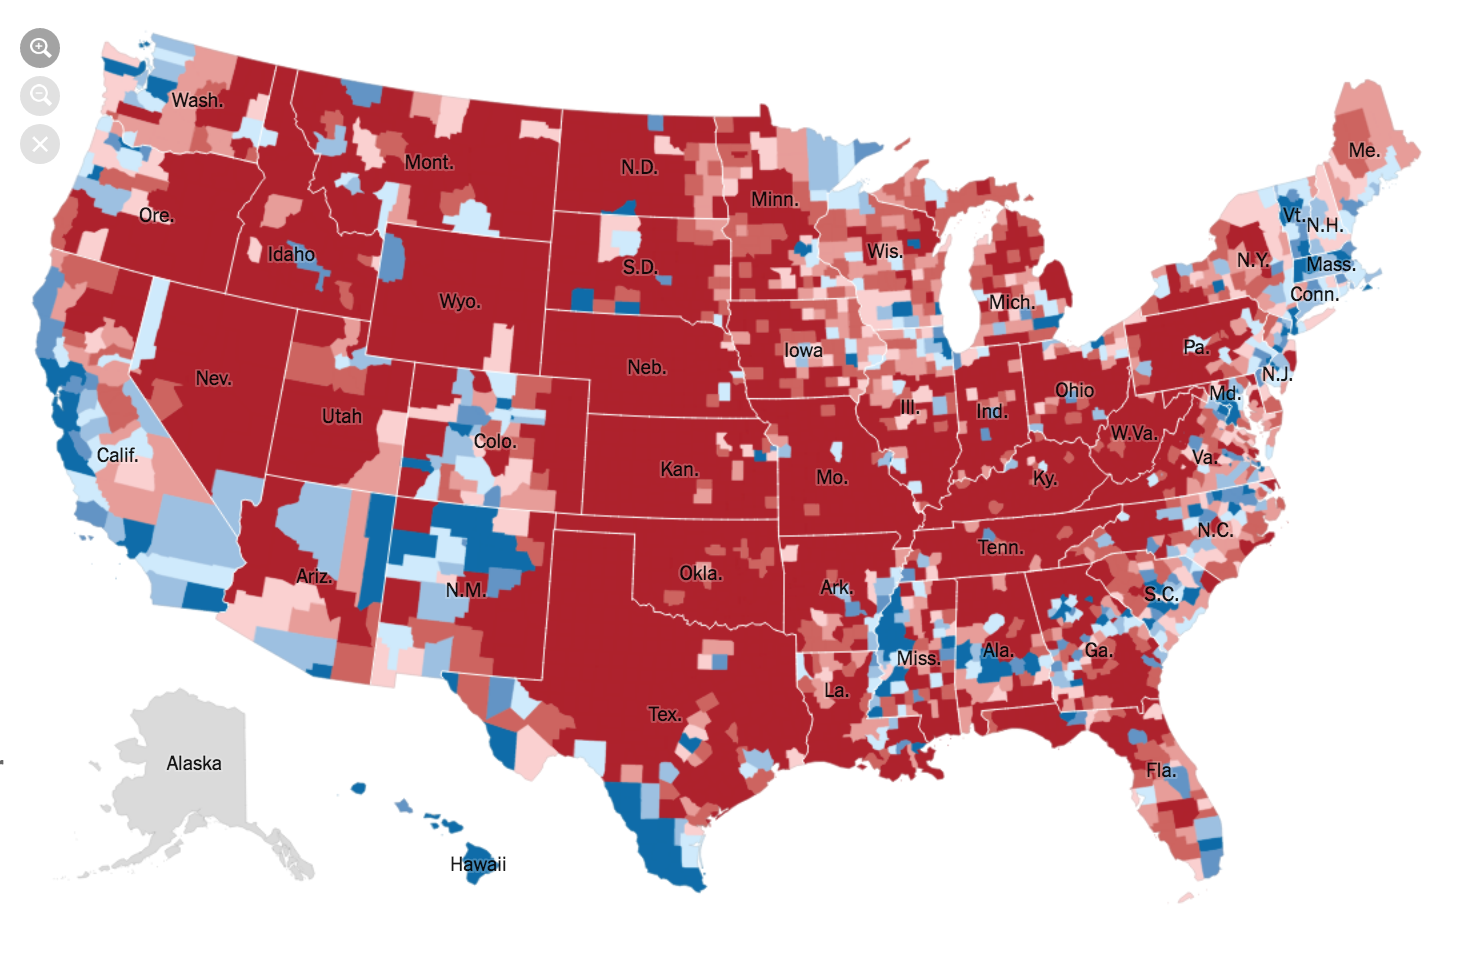
\includegraphics[width=\textwidth]{NYT}}
\end{figure}
\end{frame}

\begin{frame}
\frametitle{ALSO the United States}
\begin{figure}[H]    \centering
	{	 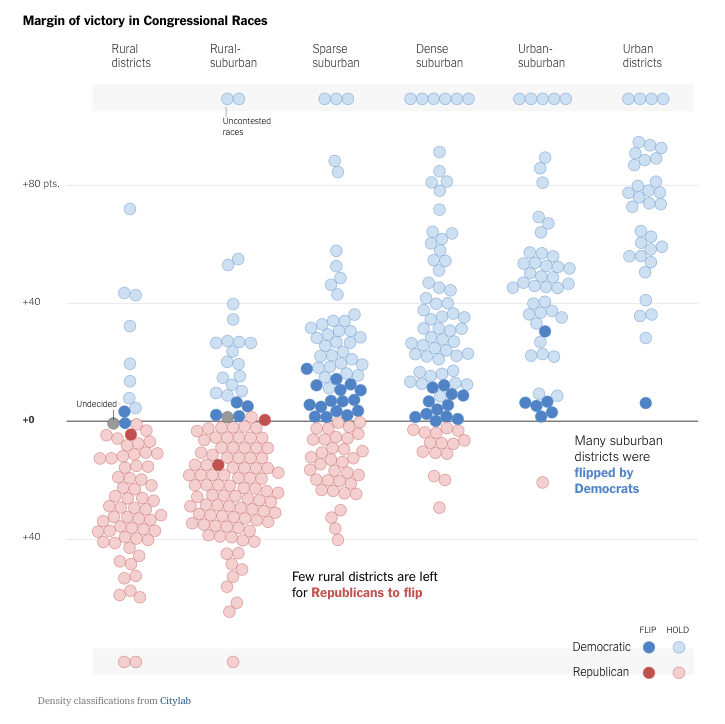
\includegraphics[width=.7\textwidth]{ClayLab}}
\end{figure}
\end{frame}

\begin{frame}
\frametitle{NOT the United States}
\begin{figure}[H]    \centering
	{	 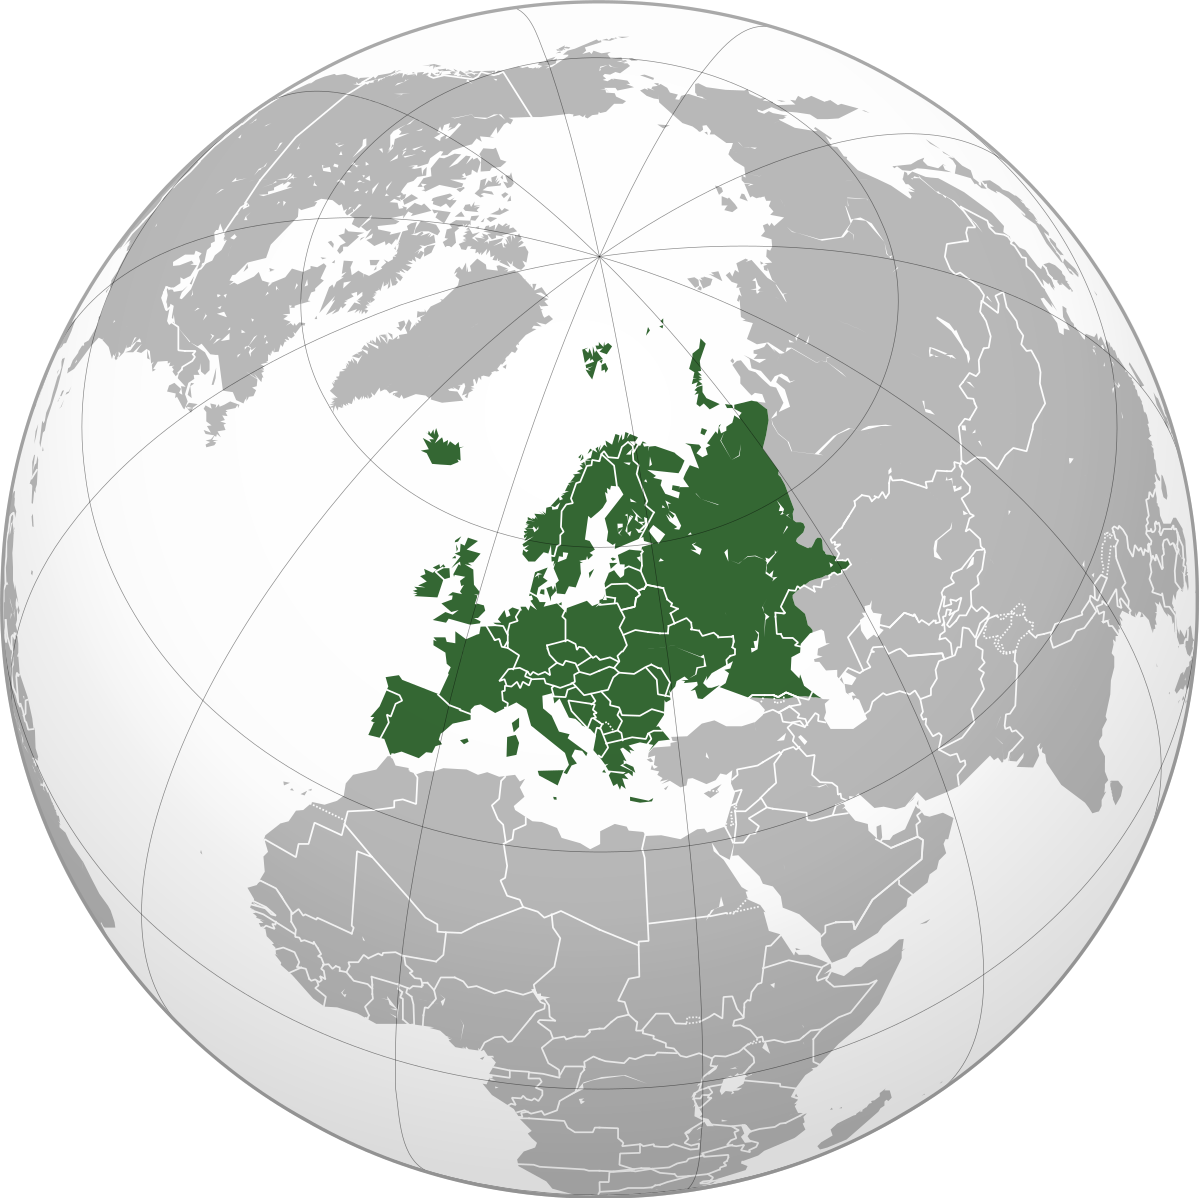
\includegraphics[width=.7\textwidth]{Europe}}
\end{figure}
\end{frame}

\begin{frame}
\frametitle{Polities to Explore}
\begin{figure}[H]    \centering
	{	 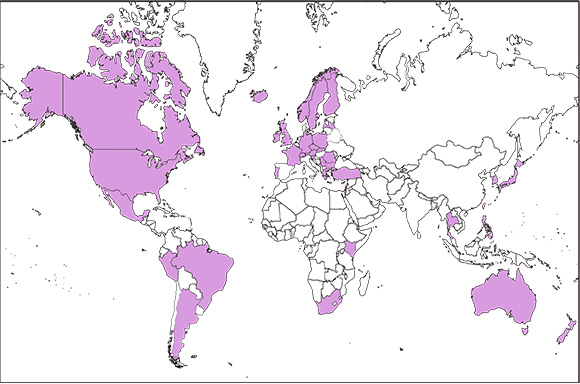
\includegraphics[width=.9\textwidth]{Mod4}}
\end{figure}
\end{frame}

\begingroup
\begin{frame}
\footnotesize
\frametitle{Hypotheses}
\e {Hypothesis 1 -- Self-Identified Ideology} \\
~~\\
\e{Hypothesis 2 -- Issue Stances} \\
~~\\
\e{Hypothesis 3A -- Level of Democracy} \\
~~\\
\e{Hypothesis 3B -- Regime Age} \\
~~\\
\e{Hypothesis 3C -- Electoral Formula}\\
~~\\
\e{Hypothesis 3D -- Polity Differences} 

\end{frame}

\begin{frame}
\frametitle{Data - CSES Module IV}
\begin{figure}[H]    \centering
	{	 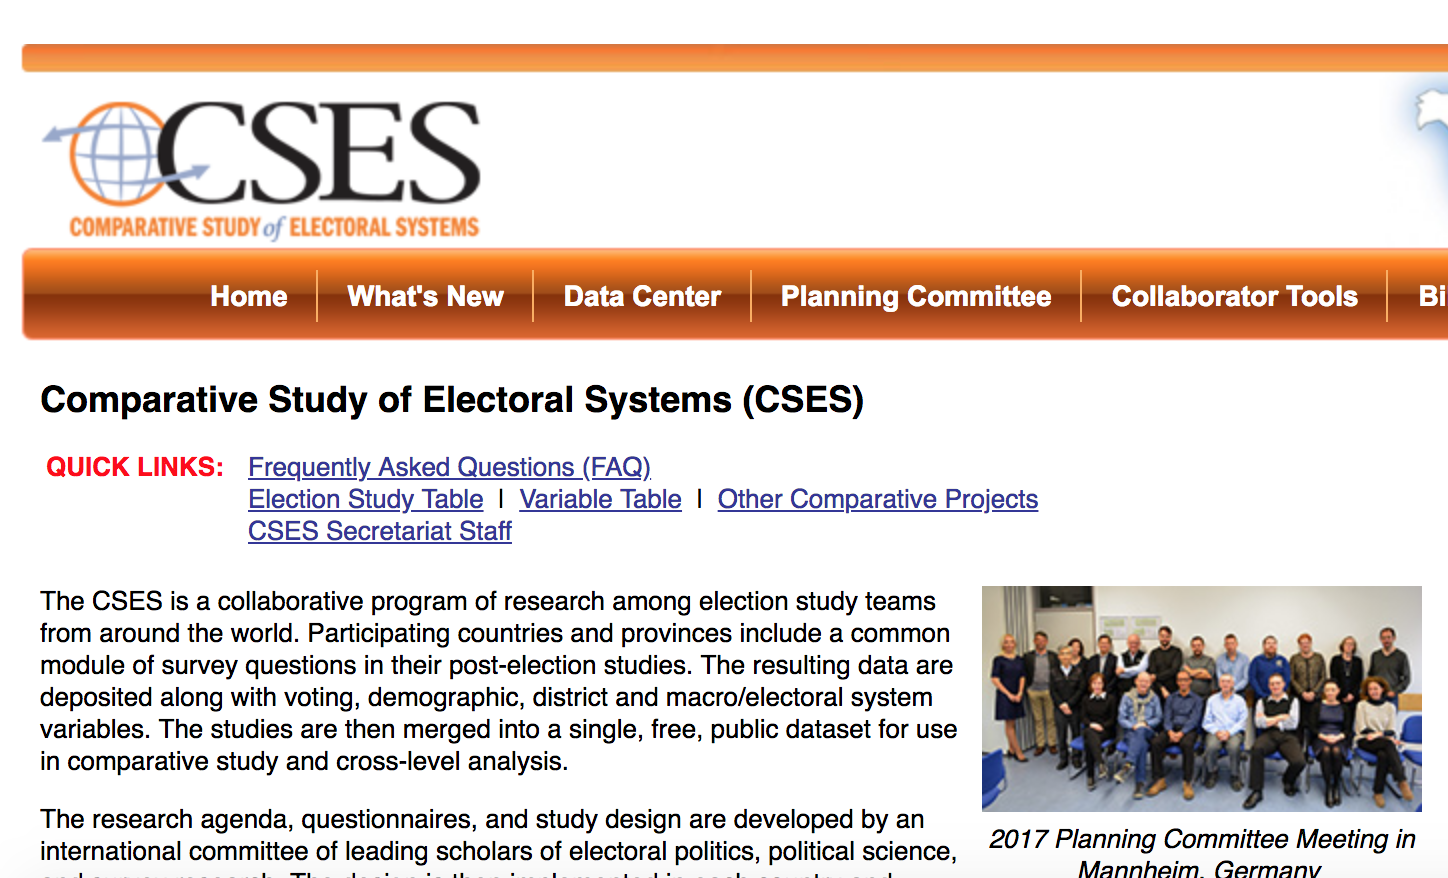
\includegraphics[width=.9\textwidth]{CSES}}
\end{figure}
\end{frame}

\begin{frame}
\frametitle{Independent Measures}
\begin{itemize}
	\item Country
	\item Place of Residence
	\item Level of Democracy
	\item Regime Age
	\item Electoral Formula
\end{itemize}
\end{frame}

\begin{frame}
\frametitle{Dependent Measures}
\begin{itemize}
	\item Self-Placement Ideology (0-10)
	\item Liberalism - Public Expenditure and Income Inequality (0-9)
\end{itemize}
\end{frame}

\begin{frame}
\frametitle{Controls}
\begin{itemize}
	\item Gender
	\item Education
	\item Socioeconomic Status
	\item Age
	\item Party Identification
	\item Closeness to Party
	\item Religiosity
\end{itemize}
\end{frame}

\begin{frame}
\normalsize
\frametitle{Models}
\begin{itemize}
	\item Self-Placement Ideology = Place of Residence + Controls
	\item Liberalism = Place of Residence + Controls
\end{itemize}
\end{frame}

\begin{frame}
\tiny
%\frametitle{Results - Ideology and Liberalism}
\begin{table}[H]
		\centering
		%\def\arraystretch{1.5}
		\caption{\tb{General Trends in Ideology}}
		\begin{tabulary}{\linewidth}{l c c}
			\\
			\hline
			\tb{Place of Residence}&\tb{Self-Placement}&\tb{Liberalism} \\
			\hline
			Small Town&.1647**&.0432  \\    
			& (..0722) &(.0278)  \\
			Suburban & .2714*** &.0082\\ 
			& (.0934) &(.0352) \\
			Urban   & .2679*** &.0995***  \\
			& (.0721)  &(.0272)  \\
			Constant   & 5.1086*** &2.7915*** \\
			&(.1993)&(.0762)  \\
			N  & 10,548 &9.662  \\
			$R^2$	& 0.0454&0.0195 \\
			\hline                                       
		\end{tabulary}
		\\
		\e{Notes:} *p$<$.1, **p$<$.05. ***p$<$.01 \\
		\e{Reference:} A rural place of residence serves as the baseline for comparison

\end{table}
\end{frame}

\begin{frame}
\frametitle{Regional Urban-Rural Splits}
\begin{figure}[H]    \centering
	{	 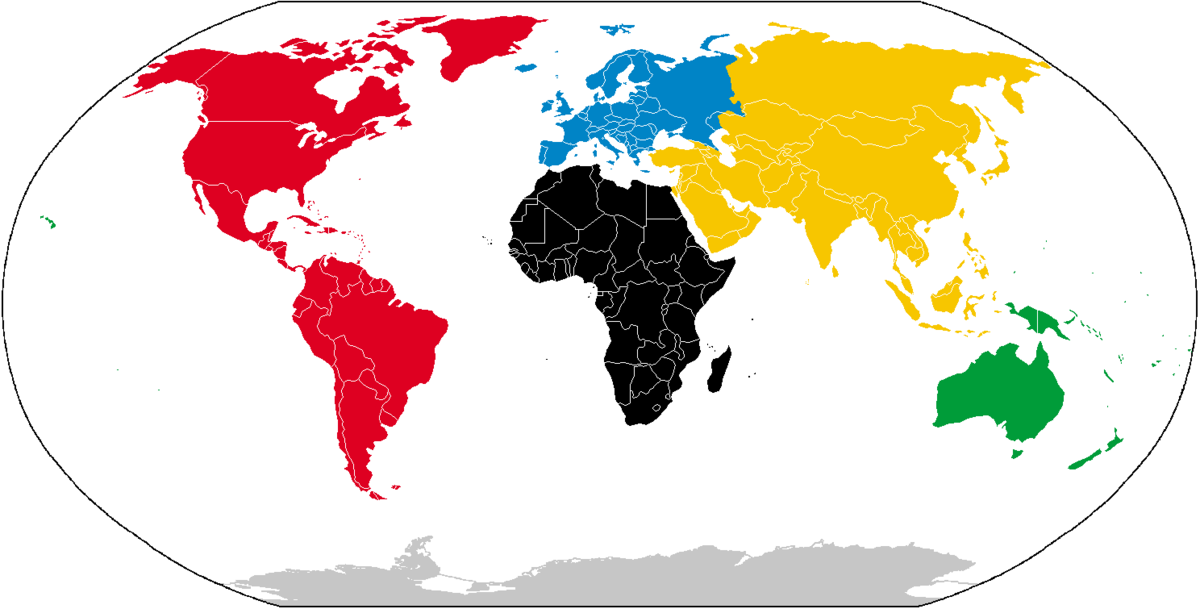
\includegraphics[width=\textwidth]{Regions}}
\end{figure}
\end{frame}

\begin{frame}
\frametitle{Macro Variables}
\begin{enumerate}
	\item Level of Democracy
	\item Regime Age
	\item Electoral Formula
\end{enumerate}	
\end{frame}

\begin{frame}
\tiny
\begin{table}[h!]
	\centering
	\caption{\tb{By Electoral Formula}}
	\begin{tabulary}{\linewidth}{l c c c}
		\\
		\hline
		\tb{Place of Residence}&\tb{Majoritarian}&\tb{Proportional} &\tb{Mixed} \\
		\hline
		Small Town&-.2413 &.3437*** &.0425 \\
		&(.1583)&(.0982) &(.1377) \\
		Suburban&-.0981 &.2715**&.4923**  \\
		&(.2307) &(.1174) &(.2124) \\
		Urban&-.3787* &.1999** &.5009*** \\
		&(.1995) &(.0981) &(.1298) \\
		Constant& 1.776*** &5.3337***&5.9321*** \\
		&(.5730) &(.2616) &(.3651) \\
		N&1,440&6,057 &3,043\\
		$R^2$&0.1375&0.0549&0.0221 \\
		\hline 
	\end{tabulary} 
	\\ 
	\e{Notes:} *p$<$.1, **p$<$.05. ***p$<$.01 \\
	\e{Reference:} A rural place of residence serves as the baseline for comparison
\end{table}
\end{frame}

\begin{frame}
\tiny
\begin{table}[h!]
	\begin{tabulary}{\linewidth}{l c c}
		\\
		\hline
		\tb{Variable}&\tb{Self-Placement}&\tb{Liberalism} \\
		\hline
		\e{Place of Residence} & & \\
		Small Town &.0231&-.0151 \\
		&(.0519)&(.0271) \\
		Suburban& .0555***& -.0777** \\
		&(.0688)& (.0350) \\
		Urban&.1214** & .0598 \\
		&(.0507) & (.0267) \\
		\e{Democracy}& -.1599*** & .0153\\
		&(.0190) & (.0088)\\
		\e{Regime Age} & .0013 & .0086***\\
		&(.00027) & (.0003)\\
		\e{Electoral Formula}&.0789*** & .0744***\\
		&(.0302) & (.0151) \\
		\hline
		Constant& 6.510*** & 2.335*** \\
		&(.2067) & (.1012)\\
		N&18,748 & 9,292 \\
		$R^2$&0.0406& 0.0930 \\
		\hline
	\end{tabulary}
	\\
	\e{Notes:} *p$<$.1, **p$<$.05. ***p$<$.01 \\
	\e{Reference:} A rural place of residence serves as the baseline for comparison
\end{table}
\end{frame}

\begin{frame}
\footnotesize
\frametitle{Hypotheses Revisited}

\e {Hypothesis 1 -- Self-Identified Ideology} \\
~~\\
\e{Hypothesis 2 -- Issue Stances} \\
~~\\
\e{Hypothesis 3A -- Level of Democracy} \\
~~\\
\e{Hypothesis 3B -- Regime Age} \\
~~\\
\e{Hypothesis 3C -- Electoral Formula}\\
~~\\
\e{Hypothesis 3D -- Polity Differences} 

\end{frame}

\begin{frame}
\frametitle{Conclusions}
\begin{figure}[H]    \centering
	{	 
\includegraphics[width=\textwidth]{RuralUrban}}
\end{figure}
\end{frame}
\endgroup

\begin{frame}
\frametitle{That's All, Folks!}
\begin{figure}[H]    \centering
	{	 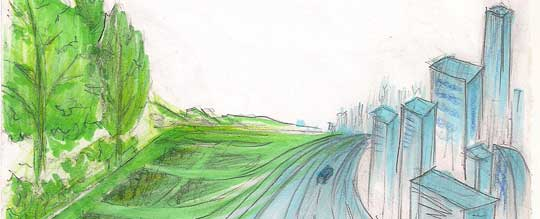
\includegraphics[width=\textwidth]{Sketch}}
\end{figure}
\end{frame}

\end{document}